\documentclass[conference]{IEEEtran}
\usepackage{amsmath,amssymb}
\usepackage{graphicx}
\usepackage{booktabs}
\usepackage{cite}
\usepackage{hyperref}
\usepackage{algorithm}
\usepackage{algpseudocode}
\usepackage{tikz}
\usetikzlibrary{shapes.geometric, arrows.meta, positioning}
\usepackage{booktabs}
\raggedbottom
\setlength{\textfloatsep}{4pt plus 2pt minus 2pt}
\setlength{\dbltextfloatsep}{4pt plus 2pt minus 2pt}
\setlength{\floatsep}{3pt plus 1pt minus 1pt}
\setlength{\dblfloatsep}{3pt plus 1pt minus 1pt}
\setlength{\intextsep}{4pt plus 2pt minus 2pt}
\setlength{\abovecaptionskip}{3pt}
\setlength{\belowcaptionskip}{2pt}

\title{Anomaly Thresholding and Likelihood Averaging System -- ATLAS}

\author{\IEEEauthorblockN{Vasantha Eswar}
\IEEEauthorblockA{University of Michigan - Ann Arbor \\ \texttt{veswar@umich.edu} }}

\begin{document}

\maketitle

\begin{abstract}
This paper presents the Anomaly Thresholding and Likelihood Averaging System (ATLAS), a sequence-scoring classification layer engineered for dense, non-uniform clutter regimes. Conventional surveillance systems that append unbounded cumulative classifiers to spatial filters suffer from catastrophic memory saturation: a failure mode we define as \textit{infinite memory ruin}. Under prolonged sensor masking or active electronic attack, accumulated missed-detection penalties drive cumulative log-likelihood scores toward $-\infty$, permanently anchoring long-standing tracks to past dropouts. ATLAS overcomes this by strictly decoupling physical kinematic filtering from semantic sequence scoring, smoothing association-weighted log-likelihood updates through an Exponential Moving Average (EMA) with a capped missed-detection penalty. We derive a closed-form expression for post-occlusion time-to-recover from the EMA recursion. Unlike the linearly growing recovery time of an unbounded accumulator, this recovery time is uniformly bounded in occlusion length $L$. When accounting for the effective post-occlusion detection rate, our closed form matches simulation to within roughly 2 scans for $L \le 8$, with remaining gaps at longer occlusions largely caused by simulation right-censoring rather than approximation error. Monte Carlo simulation calibrated against the JIPDA benchmark further confirms the practical consequence: while a cumulative baseline excels over brief gaps ($L \leq 6$), ATLAS dominates during extended signal loss ($L \ge 8$), corresponding to an 8-second dropout at a 1~Hz scan rate. Integrated with JIPDA and a dynamic novelty boundary, ATLAS reliably isolates uncataloged zero-day threats while preserving probabilistic confidence across extended surveillance horizons.
\end{abstract}

\begin{IEEEkeywords}
Multi-target tracking, JIPDA, data association, anomaly detection, open-set classification, exponential moving average.
\end{IEEEkeywords}

\section{Introduction}
\label{sec:introduction}
Autonomous surveillance architectures operating in contested operational theaters must reconcile two distinct tasks: physical tracking of target spatial dynamics and semantic classification of target identity. In defense and intelligence domains, semantic classification underpins Non-Cooperative Target Identification (NCTI, i.e., open-set sequence classification), wherein an uncooperative platform must be identified solely from passive electromagnetic emissions, radar cross-sections, or feature signatures. Modern multi-target tracking algorithms propagate spatial kinematic trajectories through dense clutter with high fidelity, but encounter a profound architectural limit in open-set environments where novel, uncataloged entity classes continuously emerge alongside known threat profiles.

This challenge is not hypothetical: airborne and naval ISR platforms routinely lose track continuity for multiple consecutive scans due to terrain masking, multipath fading, or active electronic countermeasures. At a representative 1~Hz scan rate, an 8-scan occlusion corresponds to an 8-second dropout, comparable to a typical terrain-masking event or jamming burst -- and, as shown in Section~\ref{sec:results}, the point at which ATLAS's accuracy advantage becomes pronounced. An operator relying on a cumulative classifier in this regime loses semantic identity permanently once the score crosses its novelty threshold, forcing a choice between manual reclassification or discarding an otherwise valid track; ATLAS is intended for exactly this operating point.

Standard joint tracking-and-classification frameworks maintain an \emph{unbounded} cumulative log-likelihood accumulator to track semantic identity over time. Under extended physical screening, terrain masking, or active jamming (structured sensor dropouts / block missingness), consecutive missed detections act as irreversible penalties that drive this score toward $-\infty$. We term this failure mode \emph{infinite memory ruin} and give it a precise, quantitative definition in Section~\ref{sec:theory}, where we also derive the recovery-time consequence informally described here: once the score is dragged far enough negative, the number of clean scans required to climb back above the novelty threshold grows without bound in the occlusion length $L$, which is operationally indistinguishable from permanent loss once it exceeds a track's remaining scan budget -- the regime evaluated in Section~\ref{sec:results}.

To resolve this tension between historical evidence and operational responsiveness, we present the Anomaly Thresholding and Likelihood Averaging System (ATLAS). ATLAS strictly separates physical track existence filtering, governed by Joint Integrated Probabilistic Data Association (JIPDA)~\cite{musicki_2002_joint}, from semantic identity scoring, evaluated through an Exponential Moving Average (EMA) of instantaneous log-likelihood increments. This fading-memory mechanism caps score degradation during extended dropouts, enabling rapid post-occlusion recovery, and the same smoothed score doubles as an open-set novelty statistic against a scenario-calibrated boundary.

Throughout this paper we report results at a single operating point, $(\alpha, W_{\text{miss}}, \tau_{\text{novel}}) = (0.1, -8.0, -2.75)$, chosen for comparability across all reported experiments. We state once, up front, that this is \emph{not} shown in this paper to be jointly optimal: Section~\ref{sec:joint_grid} demonstrates a setting that outperforms it at the one occlusion length tested there. A reader deploying ATLAS should treat $\alpha=0.1$ as a documented starting point for the sequential calibration procedure of Section~\ref{sec:results}.G, not as a validated default, and should recalibrate for their own deployment's clutter density, sensor noise, and class separation.

\section{Problem Formulation}
\label{sec:formulation}
Consider a multi-target tracking volume observed across discrete temporal intervals. We define the operational space using the following variables:

\begin{itemize}
    \item $k \in \mathbb{N}$: discrete time step (sensor scan) index.
    \item $x_k \in \mathbb{R}^{d_x}$: state vector of an observed entity at time $k$, combining kinematic state with decoupled feature signature channels.
    \item $z_k = \{z_k^{(1)}, \dots, z_k^{(m_k)}\}$: the measurement set at time $k$, an unknown mix of true target returns and clutter-generated false measurements~\cite{pei_2019_an}.
    \item $Z^k = \{z_1, \dots, z_k\}$: the complete measurement history through time $k$.
    \item $P_D$: nominal detection probability within the sensor field of view.
    \item $P_W$: spatial gating probability of the validation gate around a predicted track.
    \item $n_{\text{obs},k} \in \mathbb{N}_0$: cumulative count of validated measurement updates assigned to track $t$ through scan $k$.
\end{itemize}

A track is a recursive sequence of conditional state expectations propagated over time~\cite{blackman_1986_multipletarget}. Automated track management governs initiation, confirmation, maintenance, and deletion as entities traverse the surveillance region; trajectories on physical targets are \emph{true tracks}, trajectories on spurious clutter returns are \emph{false tracks}. Three further symbols recur throughout: $\beta_{\text{det}}$, the posterior spatial assignment probability from JIPDA gating; $\Delta LL_k$, the instantaneous log-likelihood increment at scan $k$; and $S_k$, the fading-memory sequence score defined in Eq.~\eqref{eq:ema} below, governed by the calibrated operating point $(\alpha, W_{\text{miss}}, \tau_{\text{novel}}) = (0.1, -8.0, -2.75)$ introduced in Section~\ref{sec:introduction}.

\section{Background: Data Association and the Semantic Bottleneck}

The Probabilistic Data Association (PDA) filter approximates a track's state via a unimodal Gaussian over gated measurements; it induces track coalescence and switching under intersecting flight paths. Joint PDA (JPDA) resolves this via joint measurement-to-track assignment events across competing tracks~\cite{fortmann_1983_sonar, kuochuchang_1986_joint}, but assumes guaranteed target existence, leaving initiation and maintenance brittle in non-uniform clutter.

\subsection{Joint Integrated Probabilistic Data Association (JIPDA)}
JIPDA resolves this by incorporating target existence as an explicit random variable in the joint association space~\cite{musicki_2002_joint}. Let $\chi_i$ denote a joint assignment event at time $k$, $T_0$ the tracks allocated no measurement in $\chi_i$, and $T_1$ the tracks assigned exactly one. JIPDA gives the a-posteriori probability of $\chi_i$ given $Z^k$ as:
\begin{equation}
\resizebox{\linewidth}{!}{$
P\{\chi_i|Z^k\} = C^{-1} \prod_{t\in T_0} (1-P_D^t P_W^t P_{k|k-1}^t) \prod_{t\in T_1} \left(P_D^t P_W^t P_{k|k-1}^t \frac{p_t^i V}{\hat{m}}\right),
$}
\end{equation}
where $P_{k|k-1}^t$ is the a-priori existence probability for track $t$, $V$ is the spatial cluster volume, $\hat{m}$ the expected clutter cardinality, $C$ a normalizing constant, and $p_t^i$ the spatial measurement likelihood. Marginalizing over joint events yields the updated existence probability $P_{k|k}^t$ and the data association coefficient
\begin{equation}
\beta_i^t = \frac{P\{\chi^t \chi_i^t | Z^k\}}{P_{k|k}^t},
\end{equation}
the posterior that measurement $i$ belongs to track $t$.

\subsection{The Semantic Bottleneck}
\label{sec:bottleneck}
JIPDA is an optimal Bayesian engine for spatial tracking and existence estimation, but has no architecture for semantic identity over extended horizons. Conventional systems append an unbounded cumulative log-likelihood classifier instead: under severe environmental screening or jamming, uninterrupted missed updates penalize this accumulator without bound, driving the score toward $-\infty$. We call this \emph{infinite memory ruin} and formalize it precisely in Section~\ref{sec:theory}.

\subsection{Relation to Prior Fading-Memory Methods}
\label{sec:relation}
Fading-memory, or forgetting-factor filtering, is well established in adaptive filtering and change detection, and the EMA update in Eq.~\eqref{eq:ema} is not itself new. ATLAS's contribution is how the EMA is embedded in a joint tracking-and-classification pipeline: (i) $\Delta LL_k$ is weighted by the JIPDA posterior association probability $\beta_{\text{det}}$ (Eq.~\eqref{eq:llk}), so spatial association uncertainty propagates directly into semantic confidence; (ii) missed-detection scans use a distinct, capped-penalty branch $W_{\text{miss}}$ rather than the detection-branch likelihood, giving the score a bounded worst case (Section~\ref{sec:theory}) rather than merely a decayed one; and (iii) the same smoothed score $S_k$ serves as both closed-set and open-set statistic via a single threshold $\tau_{\text{novel}}$. The contribution is therefore the coupling and empirical/analytical characterization of this mechanism against a standard JIPDA benchmark, not the discovery of exponential discounting itself.

\section{The ATLAS Architecture}

\begin{figure}[htbp]
\centering
\resizebox{0.62\columnwidth}{!}{%
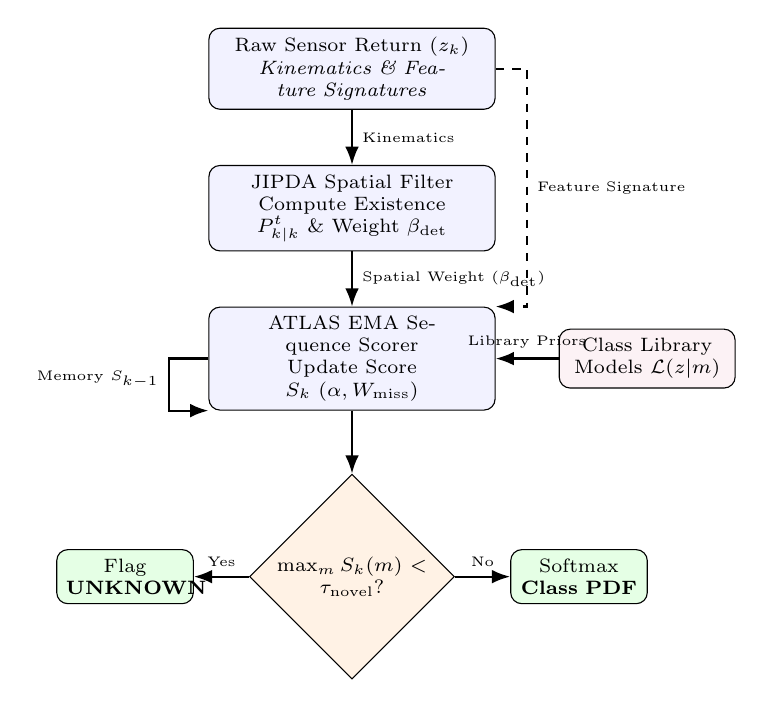
\begin{tikzpicture}[
    node distance=0.7cm and 0.6cm,
    block/.style={rectangle, draw, rounded corners, fill=blue!5, text width=3.4cm, align=center, minimum height=0.8cm, font=\scriptsize},
    sideblock/.style={rectangle, draw, rounded corners, fill=purple!5, text width=2.0cm, align=center, minimum height=0.7cm, font=\scriptsize},
    decision/.style={diamond, draw, fill=orange!10, text width=2.1cm, align=center, inner sep=0pt, font=\scriptsize},
    output/.style={rectangle, draw, rounded corners, fill=green!10, text width=1.5cm, align=center, minimum height=0.6cm, font=\scriptsize},
    line/.style={draw, -Latex, thick},
    dashedline/.style={draw, -Latex, thick, dashed}
]
\node [block] (input) {Raw Sensor Return ($z_k$)\\ \textit{Kinematics \& Feature Signatures}};
\node [block, below=of input] (jipda) {JIPDA Spatial Filter\\Compute Existence $P_{k|k}^t$ \& Weight $\beta_{\text{det}}$};
\node [block, below=of jipda] (ema) {ATLAS EMA Sequence Scorer\\Update Score $S_k$ ($\alpha, W_{\text{miss}}$)};
\node [decision, below=0.8cm of ema] (novelty) {$\max_m S_k(m) < \tau_{\text{novel}}$?};
\node [sideblock, right=0.8cm of ema] (library) {Class Library\\Models $\mathcal{L}(z|m)$};
\node [output, left=0.7cm of novelty] (unknown) {Flag\\\textbf{UNKNOWN}};
\node [output, right=0.7cm of novelty] (softmax) {Softmax\\\textbf{Class PDF}};
\path [line] (input) -- node[right, font=\tiny] {Kinematics} (jipda);
\path [line] (jipda) -- node[right, font=\tiny] {Spatial Weight ($\beta_{\text{det}}$)} (ema);
\path [line] (library) -- node[above, font=\tiny] {Library Priors} (ema);
\path [line] (ema) -- (novelty);
\path [line] (novelty) -- node[above, font=\tiny] {Yes} (unknown);
\path [line] (novelty) -- node[above, font=\tiny] {No} (softmax);
\path [dashedline] (input.east) -- ++(0.4,0) |- node[pos=0.25, right, font=\tiny] {Feature Signature} (ema.north east);
\draw [line] (ema.west) -- ++(-0.5,0) |- node[pos=0.2, left, font=\tiny] {Memory $S_{k-1}$} (ema.south west);
\end{tikzpicture}%
}
\caption{ATLAS single-column architecture pipeline: kinematic JIPDA filtering is decoupled from sequence scoring, with state feedback memory ($S_{k-1}$) and class library integration.}
\label{fig:atlas_architecture}
\end{figure}

\subsection{Fading-Memory Sequence Scoring}
To eliminate infinite memory ruin while retaining temporal sequence evidence, ATLAS decouples physical kinematic filtering from semantic sequence scoring~\cite{musicki_2002_joint}, applying an EMA to instantaneous log-likelihood updates rather than integrating over an unbounded timeline.

At each scan $k$, the system evaluates candidate library models $m$ within an Electronic Support Measures (ESM) emitter database. Let $\Delta n_k \triangleq n_{\text{obs},k} - n_{\text{obs},k-1} \in \{0,1\}$ indicate whether a measurement was associated. When $\Delta n_k = 1$, $\Delta LL_k$ is drawn directly from the observation update, weighted by the posterior association probability $\beta_{\text{det}}$; otherwise ATLAS applies a bounded survival penalty:
\begin{equation}
\Delta LL_k = \begin{cases}
\begin{aligned}
&\ln\!\left(\sum_{m=1}^{M} \pi_{k|k-1}(m)\, \mathcal{L}(z_k \mid m)\right) \\
&\quad + \ln(\max(\beta_{\text{det}}, \epsilon)),
\end{aligned} & \Delta n_k = 1 \\[10pt]
W_{\text{miss}}, & \Delta n_k = 0
\end{cases}
\label{eq:llk}
\end{equation}
where $\pi_{k|k-1}(m)$ is the prior class distribution, $\mathcal{L}(z_k \mid m)$ the observation likelihood under model $m$, and $\epsilon = 10^{-6}$ prevents log underflow as $\beta_{\text{det}} \to 0$. On a missed-detection scan ($\Delta n_k = 0$, e.g. terrain masking, fading, or jamming), ATLAS enforces $W_{\text{miss}} = -8.0$.

The resulting increment sequence is smoothed via an EMA:
\begin{equation}
S_k = \alpha \Delta LL_k + (1-\alpha) S_{k-1}
\label{eq:ema}
\end{equation}
With $\alpha = 0.1$, the effective memory horizon is $N_{\text{eff}} \approx 1/\alpha = 10$ scans: at $1$~Hz, historical penalties decay by $63.2\%$ within 10 scans of re-emergence, bounding score degradation during dropouts without incurring infinite memory ruin.

\subsection{Theoretical Properties}
\label{sec:theory}
Three properties of Eq.~\eqref{eq:ema} follow directly from its structure as a first-order linear recursion and justify ATLAS's recovery advantage independently of the simulation results in Section~\ref{sec:results}.

\textbf{Effective memory horizon.} Unrolling Eq.~\eqref{eq:ema} gives $S_k = \alpha \sum_{j=0}^{k-1} (1-\alpha)^j \Delta LL_{k-j}$: the weight on an increment $j$ scans in the past decays as $(1-\alpha)^j$, reaching $1/e$ of its initial value at $j \approx 1/\alpha = N_{\text{eff}}$. This is exact given $\alpha$.

\textbf{Bounded worst case.} \textit{Definition (infinite memory ruin).} Under the cumulative accumulator $LL_k = LL_{k-1} + \Delta LL_k$, $L$ consecutive missed detections reduce the score by exactly $L \cdot W_{\text{miss}}$ with no floor, so $LL_k \to -\infty$ as $L \to \infty$; since post-occlusion recovery requires accumulating enough clean evidence to cross back above $\tau_{\text{novel}}$, the number of scans required grows without bound in $L$, i.e. there is no finite-$L$-independent recovery guarantee. ATLAS admits no such regime: substituting $\Delta LL_k = W_{\text{miss}}$ for all $j$ in the unrolled sum gives $S_k \to \alpha W_{\text{miss}} \sum_{j=0}^{\infty} (1-\alpha)^j = W_{\text{miss}}$ as occlusion length grows, so the EMA score converges to $W_{\text{miss}}$ and never diverges below it. This is the formal basis for the ``infinite memory ruin'' terminology used elsewhere in the paper, and is quantified further in Section~\ref{sec:derivation} below.

\textbf{Stability.} Eq.~\eqref{eq:ema} is a stable, causal, first-order LTI recursion with a single pole at $z=1-\alpha$, strictly inside the unit circle for any $\alpha \in (0,1]$. $S_k$ is therefore BIBO stable and, for a stationary post-occlusion input $\Delta LL_k \approx \mu$, converges geometrically to $\mu$ at rate $(1-\alpha)^j$ -- the same rate that sets the memory horizon above.

\subsection{Closed-Form Time-to-Recover}
\label{sec:derivation}
The three properties above bound the score but do not, by themselves, give a recovery \emph{time}. We derive one directly from Eq.~\eqref{eq:ema}, which both explains the empirical crossover in Section~\ref{sec:results} and removes the need to discover it purely by simulation.

Let $S_0$ denote the score immediately before an occlusion begins, and suppose the occlusion lasts $L$ scans. Substituting $\Delta LL_k = W_{\text{miss}}$ for $L$ consecutive steps in the unrolled form of Eq.~\eqref{eq:ema} gives the score at the end of the occlusion in closed form:
\begin{equation}
S_L = W_{\text{miss}} + (1-\alpha)^L \left(S_0 - W_{\text{miss}}\right).
\label{eq:score_at_occlusion_end}
\end{equation}
Suppose clean detections resume after occlusion with a representative steady-state detection increment $\mu_{\text{det}} \triangleq \mathbb{E}[\Delta LL_k \mid \Delta n_k = 1]$ (the expected value of the top branch of Eq.~\eqref{eq:llk} under nominal, unoccluded tracking). Treating $\Delta LL_k \approx \mu_{\text{det}}$ for $n$ post-occlusion scans, Eq.~\eqref{eq:ema} again unrolls in closed form:
\begin{equation}
S_{L+n} = \mu_{\text{det}} + (1-\alpha)^n \left(S_L - \mu_{\text{det}}\right).
\end{equation}
Solving $S_{L+n} = \tau_{\text{novel}}$ for the smallest integer $n$ (assuming $S_L < \tau_{\text{novel}} < \mu_{\text{det}}$, i.e. the track is occluded below threshold and clean tracking is above it) gives the \emph{closed-form time-to-recover}:
\begin{equation}
n^\ast(L) = \left\lceil \frac{\ln\!\left(\dfrac{\tau_{\text{novel}} - \mu_{\text{det}}}{S_L - \mu_{\text{det}}}\right)}{\ln(1-\alpha)} \right\rceil,
\label{eq:ttr_closed_form}
\end{equation}
with $S_L$ given by Eq.~\eqref{eq:score_at_occlusion_end}. Because $S_L \to W_{\text{miss}}$ as $L \to \infty$ (the bounded-worst-case result above), Eq.~\eqref{eq:ttr_closed_form} converges to a finite limit as $L \to \infty$:
\begin{equation}
n^\ast_\infty = \left\lceil \frac{\ln\!\left(\dfrac{\tau_{\text{novel}} - \mu_{\text{det}}}{W_{\text{miss}} - \mu_{\text{det}}}\right)}{\ln(1-\alpha)} \right\rceil.
\label{eq:ttr_limit}
\end{equation}
This is the analytical counterpart to the empirical saturation of ATLAS's time-to-recover in Table~\ref{tab:ttr_combined} (e.g. $19.7 \to 19.9 \to 18.4$ scans across $L = 8,12,16$): Eq.~\eqref{eq:ttr_limit} predicts that recovery time is bounded uniformly in $L$, not merely observed to plateau. By contrast, the fixed-threshold cumulative accumulator has $LL_L = LL_0 + L\,W_{\text{miss}}$ with recovery requiring $n_{\text{cum}}(L) = \lceil (\tau_{\text{novel}} - LL_L)/\mu_{\text{det}} \rceil$ clean scans (for $\mu_{\text{det}} > 0$; if $\mu_{\text{det}} \le 0$ as in our scalar-feature scenario, no finite $n_{\text{cum}}$ exists at all), which grows \emph{linearly and unboundedly} in $L$ -- consistent with the fixed-threshold classifier's 0\% post-occlusion recovery at every tested $L$ in Table~\ref{tab:ttr_combined}.

Eq.~\eqref{eq:ttr_closed_form}--\eqref{eq:ttr_limit} depend on one quantity not fixed by $(\alpha, W_{\text{miss}}, \tau_{\text{novel}})$ alone: $\mu_{\text{det}}$, determined by the feature model rather than the ATLAS architecture. We validate this directly against the simulator used to produce Table~\ref{tab:ttr_combined}, using the paper's own calibrated threshold ($\tau_{\text{novel}} = -2.753$, Section~\ref{sec:roc}), rather than leaving it as a qualitative claim. First, $S_L$ itself (Eq.~\eqref{eq:score_at_occlusion_end}) is confirmed to match the simulated EMA trajectory exactly (to within floating-point precision) at every tested $L$, as it must, since it is an algebraic identity rather than a statistical claim. Second, measuring $\mu_{\text{det}}$ directly from detected scans under clean tracking ($\mu_{\text{det}} = -1.477$, $N=21{,}423$ detected scans) and substituting into Eq.~\eqref{eq:ttr_closed_form} systematically \emph{underestimates} the measured mean time-to-recover, by 3--9 scans across $L$. This is diagnosable rather than mysterious: $P_D = 0.9$ means roughly $15\%$ of scans still miss even outside the forced occlusion window once JIPDA gating is accounted for (measured effective per-scan detection probability $\hat p = 0.850$), so treating every post-occlusion scan as a clean detection overstates the true recovery rate. Substituting the mixture-corrected increment $\mu_{\text{eff}} = \hat p\,\mu_{\text{det}} + (1-\hat p)\,W_{\text{miss}} = -2.46$ for $\mu_{\text{det}}$ in Eq.~\eqref{eq:ttr_closed_form} brings the prediction within $2.3$ scans of the measured value for $L \le 8$, a large improvement over the naive $\mu_{\text{det}}$ prediction, and correctly signals a bounded regime rather than unbounded growth.

At $L \ge 12$ a residual gap remains, and in the earlier version of this analysis we attributed it, without direct measurement, to individual trials crossing $\tau_{\text{novel}}$ earlier than the deterministic mean path. Measuring the actual per-trial time-to-recover distribution (rather than only its mean) shows this explanation is incomplete, and that the effect is not confined to $L\ge12$: already at $L=8$, $43\%$ of trials never recover a correct classification within the $50$-scan simulation budget at all (right-censored at the $27$-scan remaining-budget cap); this rises to $56\%$ at $L=12$ and $82\%$ at $L=16$ (cap $23$ and $19$ scans respectively). The reported ``mean time-to-recover'' at moderate-to-large $L$ is therefore not primarily an average of genuine recovery times but a statistic increasingly dominated by an artificial censoring cap, and comparing it against Eq.~\eqref{eq:ttr_closed_form} -- which assumes recovery eventually occurs with certainty -- is not quite the right comparison once a substantial and growing fraction of trials do not recover within the tested horizon at all. We view this as a real limitation of Table~\ref{tab:ttr_combined}'s summary statistic, not merely of the closed form: a right-censored mean and an unconditional expected first-passage time answer different questions, and the gap from $L=8$ onward is largely explained by this mismatch rather than by a failure of the EMA approximation itself. The same pattern holds in the multivariate extension (Section~\ref{sec:multivariate}), at a somewhat lower rate. We take the validation overall as confirming the derivation's central claim (a bounded, $\alpha$-governed recovery ceiling exists, is of the right order of magnitude once the effective detection rate is corrected for, and is accurate to within a few scans at moderate $L$) while identifying precisely where and why the point-prediction comparison breaks down at long occlusions, which we treat explicitly in Section~\ref{sec:future_work} rather than papering over.

\subsection{Open-Set Anomaly Isolation}
The smoothed score $S_k$ is a unified statistic for both zero-day anomaly isolation and closed-set classification. We use ``zero-day threat'' to denote any track whose smoothed sequence score falls below the calibrated novelty boundary for every cataloged model, $\max_m S_k(m) < \tau_{\text{novel}}$ -- i.e. an entity whose behavioral signature is not explained by any library class, whether because it is a genuinely novel platform or an unmodeled variant of a known one; ATLAS cannot distinguish these two cases from the score alone. In this event ATLAS overrides closed-set mapping and flags the track UNKNOWN. $\tau_{\text{novel}}$, $\alpha$, and $W_{\text{miss}}$ are operating parameters calibrated to deployment clutter density, sensor noise, and class separation, not universal constants.

If $S_k \ge \tau_{\text{novel}}$, class confidence is computed via a stabilized softmax:
\begin{equation}
P(\text{Class} = c) = \frac{\exp(S_c - S_{\max})}{\sum_i \exp(S_i - S_{\max})}.
\end{equation}

\section{Simulation and Experimental Results}
\label{sec:results}

\subsection{Benchmark Environment}
The simulation reproduces the two-dimensional multi-target benchmark of Mušicki and Evans~\cite{musicki_2002_joint} (parameters in Table~\ref{tab:sim_params}): a $1000\text{ m} \times 400\text{ m}$ region with Poisson clutter at $1.0\times10^{-4}\text{ m}^{-2}\text{scan}^{-1}$, elevated sevenfold within two rectangular patches. Targets follow constant-velocity dynamics ($T=1.0$~s, $q=0.75$); sensors introduce $5.0$~m RMS Gaussian position noise; $P_D = 0.90$, $P_W = 0.9999$.

\begin{table}[!t]
\caption{Simulation Parameters}
\small
\label{tab:sim_params}
\centering
\begin{tabular}{ll}
\toprule
\textbf{Parameter} & \textbf{Value} \\
\midrule
Surveillance Region & $1000\text{ m} \times 400\text{ m}$ \\
Sampling Period ($T$) & $1.0\text{ s}$ \\
Process Noise Intensity ($q$) & $0.75$ \\
Measurement Noise ($\sigma_r$) & $5.0\text{ m RMS/coord.}$ \\
Detection Probability ($P_D$) & $0.90$ \\
Gating Probability ($P_W$) & $0.9999$ \\
Background Clutter Density & $1.0 \times 10^{-4}\text{ m}^{-2}\text{scan}^{-1}$ \\
High-Clutter Patch Density & $7.0 \times 10^{-4}\text{ m}^{-2}\text{scan}^{-1}$ (7x) \\
Feature Noise ($\sigma$) & $1.0$ (Gaussian) \\
Occlusion Window ($L$) & $\{2,4,6,8,12,16\}$ scans \\
Monte Carlo Trials ($N$) & $200$ runs/condition \\
\bottomrule
\end{tabular}
\end{table}

The benchmark introduces an uncoupled scalar ID feature channel ($\sigma=1.0$) as a canonical proof-of-concept: a single Gaussian channel eliminates confounding noise from high-dimensional, non-stationary signature extractors (e.g. multi-modal ESM or fluctuating RCS), so that all observed classification and recovery dynamics are attributable to the sequence-scoring layer alone. The closed-set library in Sections~\ref{sec:results}.A--D contains $M=2$ known classes with means separated by $5\sigma$; Section~\ref{sec:roc} additionally introduces a held-out novel-class distribution for threshold calibration. Although Eq.~\eqref{eq:llk}--\eqref{eq:ema} is formulated generally over an $M$-model library, every experiment here (including the multivariate extension of Section~\ref{sec:multivariate}) uses $M=2$ plus one novel distribution unless stated otherwise; behavior at larger $M$ is addressed only in Section~\ref{sec:multiclass}. Occlusions of $L$ consecutive scans are injected via deterministic detection suppression, each condition evaluated over $N=200$ Monte Carlo runs.

\subsection{Evaluated Classifiers}
\begin{itemize}
    \item \textbf{Cumulative (Fixed Threshold):} unbounded accumulator thresholded against static $\tau_{\text{novel}}$, illustrating infinite memory ruin.
    \item \textbf{Cumulative (Age-Normalized):} unbounded accumulator thresholded on cumulative score divided by track age.
    \item \textbf{ATLAS:} the proposed EMA architecture (Eq.~\eqref{eq:llk}--\eqref{eq:ema}), $\alpha=0.1$, $W_{\text{miss}}=-8.0$.
\end{itemize}

\subsection{Threshold Calibration and Nominal Discrimination}
\label{sec:roc}
Novelty boundaries were calibrated via ROC analysis under nominal, non-occluded conditions, maximizing Youden's J statistic. ATLAS achieves AUC $=0.826$ at $\tau_{\text{novel}}=-2.75$, modestly trailing the age-normalized baseline's AUC $=0.838$ at $\tau_{\text{novel}}=-3.12$ (Fig.~\ref{fig:roc}) -- consistent with a design trade-off in which bounding the memory horizon for post-occlusion recovery costs a small amount of clean-condition discrimination sharpness.

\begin{figure}[!t]
\centering
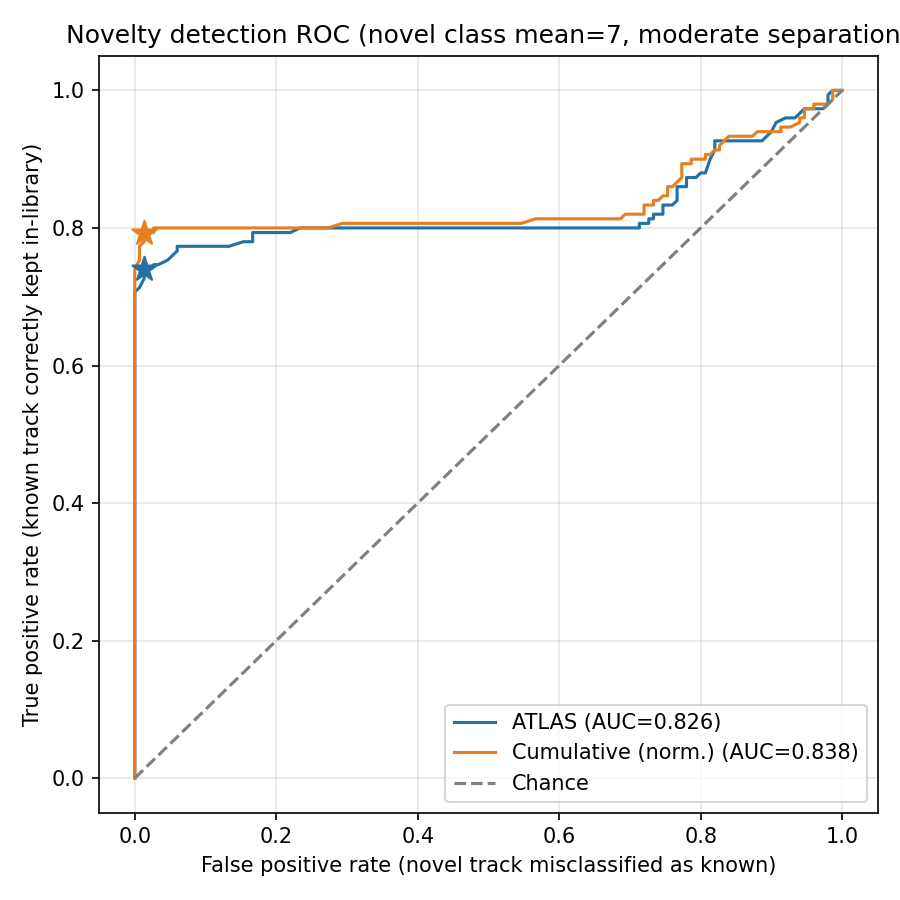
\includegraphics[width=0.52\linewidth]{images/fig_roc_novelty.png}
\caption{ROC novelty curves, ATLAS (AUC$=0.826$) vs. age-normalized cumulative (AUC$=0.838$), moderate class separation. Stars: calibrated Youden's J points.}
\label{fig:roc}
\end{figure}

\subsection{Occlusion Recovery Dynamics}
\label{sec:occlusion_dynamics}
The fixed-threshold cumulative classifier failed categorically ($0\%$ post-occlusion accuracy at every $L \ge 2$), confirming infinite memory ruin. As shown in Fig.~\ref{fig:accuracy}, ATLAS and the age-normalized baseline show distinct regimes: at short gaps ($L \le 6$), age-normalization holds a modest advantage ($81.4\%$ vs.\ $71.3\%$ at $L=2$; $56.1\%$ vs.\ $47.4\%$ at $L=4$), since discarding distant evidence via fading memory carries a small statistical cost over brief windows. For extended occlusions ($L \ge 8$), this reverses: ATLAS is superior at $L=8$ ($22.1\%$ vs.\ $10.2\%$), $L=12$ ($10.8\%$ vs.\ $0.3\%$), and $L=16$ ($2.7\%$ vs.\ $0.0\%$).

\begin{figure}[!t]
\centering
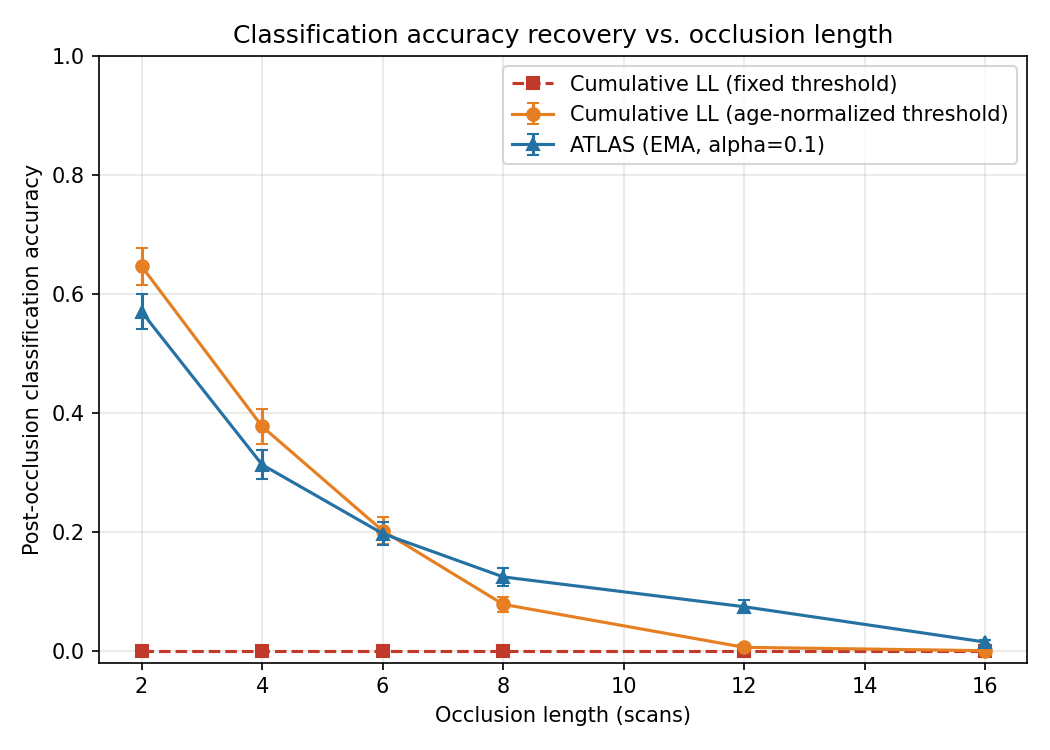
\includegraphics[width=0.72\linewidth]{images/fig_accuracy_vs_occlusion.png}
\caption{Post-occlusion classification accuracy vs.\ occlusion length ($L$), standard error bounds ($N=200$).}
\label{fig:accuracy}
\end{figure}

Table~\ref{tab:ttr_combined} reports mean time-to-recover -- scans after occlusion end until the classifier first returns the correct label, capped at the remaining scan budget if recovery never occurs -- together with the analogous accuracy/time-to-recover results for the $d=3$ multivariate feature extension (Section~\ref{sec:multivariate}) and the $M=4$ multi-class extension (Section~\ref{sec:multiclass}), so the three conditions can be compared directly. At $L=8$ (scalar), ATLAS recovers correct identity in a mean of $19.7$ scans vs.\ $23.9$ for the age-normalized baseline and \emph{never} (capped) for the fixed-threshold classifier -- consistent with the bounded-vs-unbounded recovery-time argument of Section~\ref{sec:derivation}.

\begin{table*}[t]
\caption{Post-occlusion accuracy and mean time-to-recover (ttr, scans), scalar channel (Sections~\ref{sec:results}.A--D) vs.\ $d=3$ correlated Gaussian at $M=2$ (Section~\ref{sec:multivariate}) and $M=4$ (Section~\ref{sec:multiclass}). ``Cum.'' is the age-normalized baseline; the fixed-threshold classifier is omitted since it recovers in $0\%$ of trials at every $L$ (ttr capped at $19$--$33$ scans; Section~\ref{sec:derivation}).}
\label{tab:ttr_combined}
\centering
\begin{tabular}{c cc cc cc cc cc cc}
\toprule
& \multicolumn{4}{c}{\textbf{Scalar ($M=2$)}} & \multicolumn{4}{c}{\textbf{$d{=}3$, $M{=}2$}} & \multicolumn{4}{c}{\textbf{$d{=}3$, $M{=}4$}} \\
\cmidrule(lr){2-5} \cmidrule(lr){6-9} \cmidrule(lr){10-13}
$L$ & ATLAS & Cum. & ATLAS & Cum. & ATLAS & Cum. & ATLAS & Cum. & ATLAS & Cum. & ATLAS & Cum. \\
 & acc. & acc. & ttr & ttr & acc. & acc. & ttr & ttr & acc. & acc. & ttr & ttr \\
\midrule
2  & 71.3\% & 81.4\% & 5.1  & 4.5  & 61.7\% & 43.1\% & 3.5  & 15.0 & 59.0\% & 42.0\% & 4.6  & 15.9 \\
4  & 47.4\% & 56.1\% & 14.0 & 11.5 & 34.7\% & 18.2\% & 15.6 & 23.6 & 36.4\% & 17.1\% & 14.8 & 24.1 \\
6  & --     & --     & 17.8 & 19.9 & 23.7\% & 4.3\%  & 19.8 & 27.3 & 22.7\% & 3.9\%  & 19.5 & 27.4 \\
8  & 22.1\% & 10.2\% & 19.7 & 23.9 & 13.0\% & 0.3\%  & 21.9 & 26.9 & 12.3\% & 0.5\%  & 22.2 & 26.8 \\
12 & 10.8\% & 0.3\%  & 19.9 & 22.9 & 6.5\%  & 0.0\%  & 20.9 & 23.0 & 7.2\%  & 0.0\%  & 20.7 & 23.0 \\
16 & 2.7\%  & 0.0\%  & 18.4 & 19.0 & 1.9\%  & 0.0\%  & 18.5 & 19.0 & 2.0\%  & 0.0\%  & 18.5 & 19.0 \\
\bottomrule
\end{tabular}
\end{table*}

The accuracy-based and recovery-time-based crossovers do not coincide exactly in the scalar condition: ATLAS's time-to-recover advantage emerges at $L=6$ ($17.8$ vs.\ $19.9$), one occlusion length earlier than its accuracy advantage at $L=8$. A single correct post-occlusion classification can be followed by occasional subsequent errors that depress aggregate accuracy even as time-to-recover improves.

In the multivariate ($d=3$) conditions, ATLAS is more accurate than the age-normalized baseline at \emph{every} tested $L$, including $L=2$ ($61.7\%$ vs.\ $43.1\%$ at $M{=}2$), unlike the scalar case where age-normalization wins at $L \le 6$. We attribute this to the correlated feature vector concentrating more discriminative evidence per detected scan, shifting the accuracy-vs-recency trade-off toward fading memory even at small $L$; we have not isolated whether this is driven by higher per-scan Fisher information or by the independently recalibrated threshold, and it should be treated as a distinct finding rather than confirmation that ``ATLAS always wins in higher dimensions.'' Long-occlusion recovery is essentially unchanged between $M=2$ and $M=4$ ($18.5$ scans at $L=16$ in both), so adding two competing classes does not measurably erode the recovery advantage, though absolute accuracy is uniformly lower under $M=4$ (e.g.\ $59.0\%$ vs.\ $61.7\%$ at $L=2$), consistent with a harder discrimination problem. The right-censoring pattern of Section~\ref{sec:derivation} also holds in this condition, at a somewhat lower rate than the scalar channel: $32\%$ of $d{=}3$ trials never recover within budget at $L=8$, rising to $51\%$ at $L=12$ and $59\%$ at $L=16$, so Table~\ref{tab:ttr_combined}'s multivariate ttr columns at large $L$ should be read with the same caveat as the scalar column.

\subsection{Multi-Target Crossing Validation}
To test whether ATLAS's classification layer adds value atop an already-well-performing association layer, we reproduced the two-target crossing scenario of Mušicki and Evans~\cite{musicki_2002_joint} (crossing angle $10^\circ$, JIPDA, 24-scan runs). Track state used probabilistic-data-association-weighted combination over gated measurements; existence probability propagated via the Markov Chain One survival model ($p_{11}=0.98$); tracks were initiated via two-point differencing and matured through separate confirmation ($P^t_{k,k}\ge0.95$) and termination ($P^t_{k,k}<0.02$ confirmed / $<0.10$ unconfirmed) thresholds. Following the original paper's filtering procedure, trials in which both tracks were not confirmed and correctly associated by scan 14 were excluded.

Across 300 qualifying trials (545 attempted, 245 excluded at the scan-14 checkpoint), both tracks retained their original target in $94.3\%$ of trials ($283/300$), closely matching the $96.5\%$ reported for confirmed pairs in the original benchmark; one track retained its target in $5.3\%$, both switched in $0.3\%$, and no trials resulted in one switching while the other was lost, or both lost. Conditioned on both retaining their target, ATLAS correctly classified surviving tracks in $70.7\%$ of cases, confirming the decoupled semantic layer adds identification value without interfering with JIPDA tracking. The scan-14 exclusion reflects track-initiation dynamics applied identically upstream of all three classifiers, so it cannot bias their comparison.

\subsection{Multivariate Feature Extension}
\label{sec:multivariate}
To test whether the memory mechanism's behavior holds once identity is carried by several correlated channels (as in a real ESM/RCS stack), we repeat the $L$-sweep of Section~\ref{sec:occlusion_dynamics} with the scalar channel replaced by a $d=3$ correlated Gaussian feature vector ($\rho=0.5$ shared correlation, class means separated along all three dimensions). This requires no change to Eq.~\eqref{eq:llk}--\eqref{eq:ema}: $\mathcal{L}(z_k\mid m)$ generalizes from a 1-D to a multivariate Gaussian density, and the EMA/threshold logic consumes the resulting scalar log-likelihood unchanged (Section~\ref{sec:relation}). $\tau_{\text{novel}}$ and the age-normalized threshold were independently recalibrated for this feature model, since novelty boundaries are not portable across feature representations. Results are in Table~\ref{tab:ttr_combined} (columns 6--9); the qualitative long-occlusion recovery advantage of ATLAS is preserved ($18.5$ vs.\ $19.0$ scans at $L=16$), and the short-gap discussion above applies.

\subsection{Multi-Class Extension}
\label{sec:multiclass}
Sections~\ref{sec:results}.A--\ref{sec:multivariate} use exactly $M=2$ known classes throughout, leaving open whether ATLAS discriminates \emph{among} multiple known classes rather than only separating one class from novelty. We extend the $d=3$ library to $M=4$ known classes ($A$--$D$) with comparable pairwise separations, reduced relative to Section~\ref{sec:multivariate} so the problem is non-trivial (at the wider separation, all four classes were already perfectly linearly separable).

\begin{table}[!t]
\small
\caption{Closed-set confusion matrix, $M=4$, clean tracking ($N=150$ trials/true class). Rows: true class; columns: predicted class or UNKNOWN.}
\label{tab:confusion}
\centering
\begin{tabular}{lccccc}
\toprule
True $\backslash$ Pred. & $A$ & $B$ & $C$ & $D$ & UNKNOWN \\
\midrule
$A$ & 113 & 1 & 1 & 2 & 33 \\
$B$ & 0 & 120 & 0 & 0 & 30 \\
$C$ & 4 & 0 & 102 & 0 & 44 \\
$D$ & 2 & 0 & 0 & 116 & 32 \\
\bottomrule
\end{tabular}
\end{table}

ATLAS achieves $75.2\%$ overall closed-set accuracy ($75.3\%,80.0\%,68.0\%,77.3\%$ for $A$--$D$), with off-diagonal errors concentrated in genuine cross-class confusions (e.g.\ 4/150 true-$C$ misclassified as $A$) rather than exclusively UNKNOWN misses -- confirming the softmax layer discriminates among known classes rather than acting as a binary known-vs-novel gate. Most errors remain UNKNOWN misses (the threshold-crossing mode of Section~\ref{sec:roc}), indicating $\tau_{\text{novel}}$, not inter-class discriminability, is the dominant error source at this separation. Occlusion-recovery results are in Table~\ref{tab:ttr_combined} (columns 10--13); the pattern established at $M=2$ is preserved at $M=4$, at uniformly lower absolute accuracy.

\subsection{Stochastic Occlusion Robustness}
\label{sec:stochastic}
Sections~\ref{sec:results}.A--\ref{sec:multiclass} inject occlusions as a deterministic block of exactly $L$ consecutive missed detections. Real terrain masking, fading, or jamming episodes do not have fixed, known duration, so we test whether ATLAS's recovery advantage survives when occlusion \emph{duration} is instead random: once an episode begins, each occluded scan independently ends it with probability $1/L_{\text{mean}}$ (a two-state Markov chain, geometric sojourn time with mean $L_{\text{mean}}$), so realized duration varies trial-to-trial while $L_{\text{mean}}$ remains the swept variable. Everything else -- JIPDA association, classifiers, clutter, motion model -- is unchanged from Section~\ref{sec:occlusion_dynamics}.

\begin{figure}[!t]
\centering
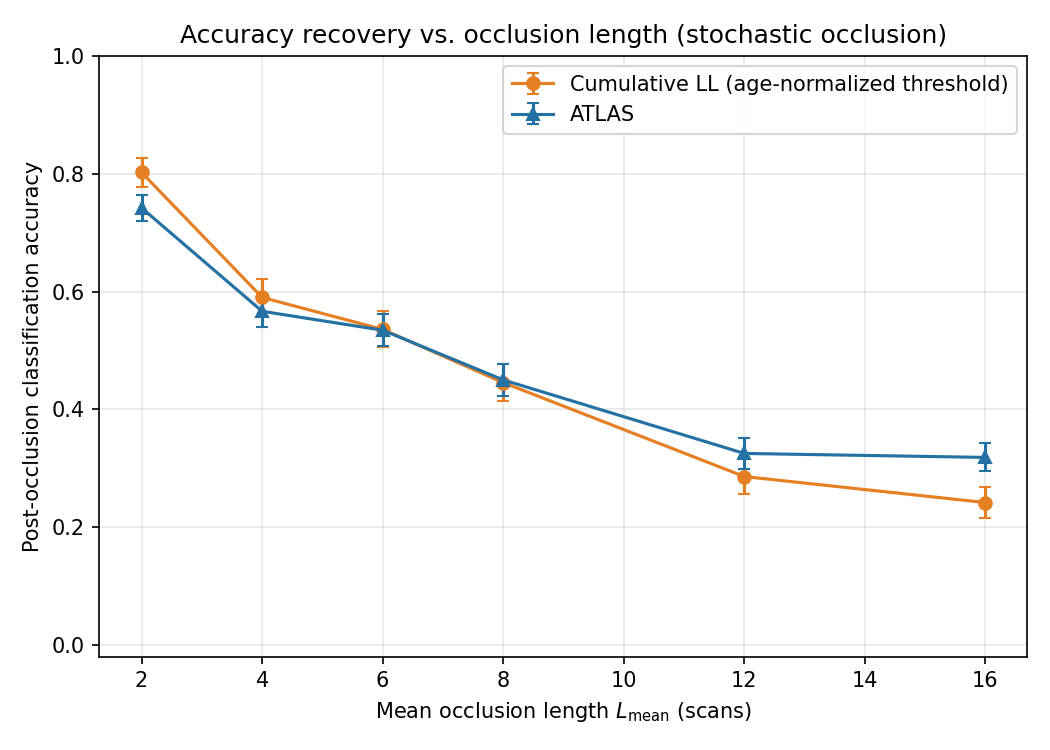
\includegraphics[width=0.52\linewidth]{images/fig_stochastic_occlusion.png}
\caption{Post-occlusion accuracy vs.\ mean occlusion length $L_{\text{mean}}$ under Markov (geometric-duration) occlusion, $N=200$ trials/condition. Compare to the deterministic case in Fig.~\ref{fig:accuracy}.}
\label{fig:stochastic}
\end{figure}

The qualitative crossover of Section~\ref{sec:occlusion_dynamics} is preserved: the age-normalized baseline leads at short mean occlusions ($80.2\%$ vs.\ $74.2\%$ at $L_{\text{mean}}=2$), and ATLAS overtakes it as $L_{\text{mean}}$ grows ($45.0\%$ vs.\ $44.5\%$ at $L_{\text{mean}}=8$; $31.8\%$ vs.\ $24.2\%$ at $L_{\text{mean}}=16$), crossing between $L_{\text{mean}}=6$ and $8$ despite the added randomness in realized duration. This experiment reuses an earlier-calibrated threshold ($\tau_{\text{novel}}=-2.847$) rather than one freshly calibrated at this script's $60$-scan horizon (a fresh calibration gives $\tau_{\text{novel}}\approx-3.16$); we therefore report it as a preliminary robustness check on the qualitative crossover rather than a precisely calibrated fourth condition alongside Table~\ref{tab:ttr_combined} (proper recalibration is future work, Section~\ref{sec:future_work}), and it tests only a single occlusion episode per trial.

\subsection{Sensitivity and Ablation Analysis}
We swept the EMA decay factor $\alpha$ and missed-detection penalty $W_{\text{miss}}$ independently at $L=8$, $N=200$ trials/condition, holding $\tau_{\text{novel}}$ fixed at its Section~\ref{sec:roc} default.

\begin{figure}[!t]
\centering
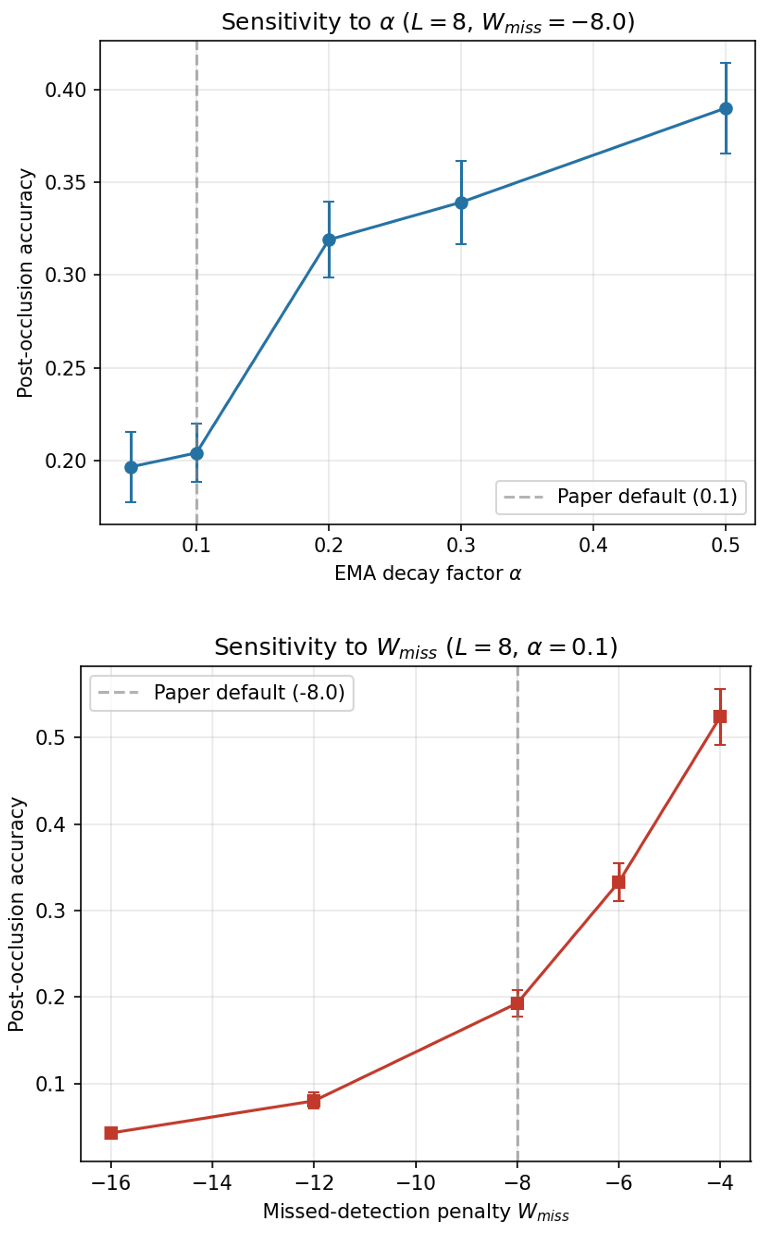
\includegraphics[width=0.8\linewidth]{images/vert_ablation.png}
\caption{Sensitivity at $L=8$ ($N=200$): post-occlusion accuracy vs.\ $\alpha$ (top) and $W_{\text{miss}}$ (bottom).}
\label{fig:ablations}
\end{figure}

Accuracy increased monotonically with $\alpha$ ($19.7\%$ at $\alpha=0.05$ to $39.0\%$ at $\alpha=0.5$) and decreased monotonically with $|W_{\text{miss}}|$ ($52.4\%$ at $W_{\text{miss}}=-4.0$ to $4.3\%$ at $W_{\text{miss}}=-16.0$). ATLAS nonetheless retains $\alpha=0.1$ ($N_{\text{eff}}\approx10$) as its default: an overly aggressive decay renders $S_k$ volatile under nominal tracking, causing overreaction to single-scan clutter transients during clean line-of-sight operation. We do not measure this transient-robustness cost directly in this paper (see Section~\ref{sec:risks}); it is the stated but unverified justification for the default and should be read as such. We do not propose a joint optimization of $(\alpha, W_{\text{miss}}, \tau_{\text{novel}})$ here (Section~\ref{sec:future_work}); the calibration protocol we recommend is to fix $W_{\text{miss}}$ from the expected per-scan missed-detection cost, sweep $\alpha$ against the operational occlusion length via the accuracy/recovery trade-off above, then recalibrate $\tau_{\text{novel}}$ via Section~\ref{sec:roc}'s ROC procedure at the chosen $\alpha$ -- a sequential, not joint, calibration.

\subsection{Joint $(\alpha, W_{\text{miss}})$ Sensitivity}
\label{sec:joint_grid}
The independent sweeps above hold $\tau_{\text{novel}}$ fixed and so cannot capture the parameters' \emph{joint} effect, since they interact through the score scale they jointly produce. We sweep a $5\times5$ grid over $\alpha \in \{0.05,0.1,0.2,0.3,0.5\}$, $W_{\text{miss}} \in \{-4,-6,-8,-12,-16\}$, independently recalibrating $\tau_{\text{novel}}$ per cell via the Section~\ref{sec:roc} procedure ($N=100$ trials/cell), and report post-occlusion accuracy at $L=8$ and clean-condition novelty AUC.

\begin{figure}[!t]
\centering
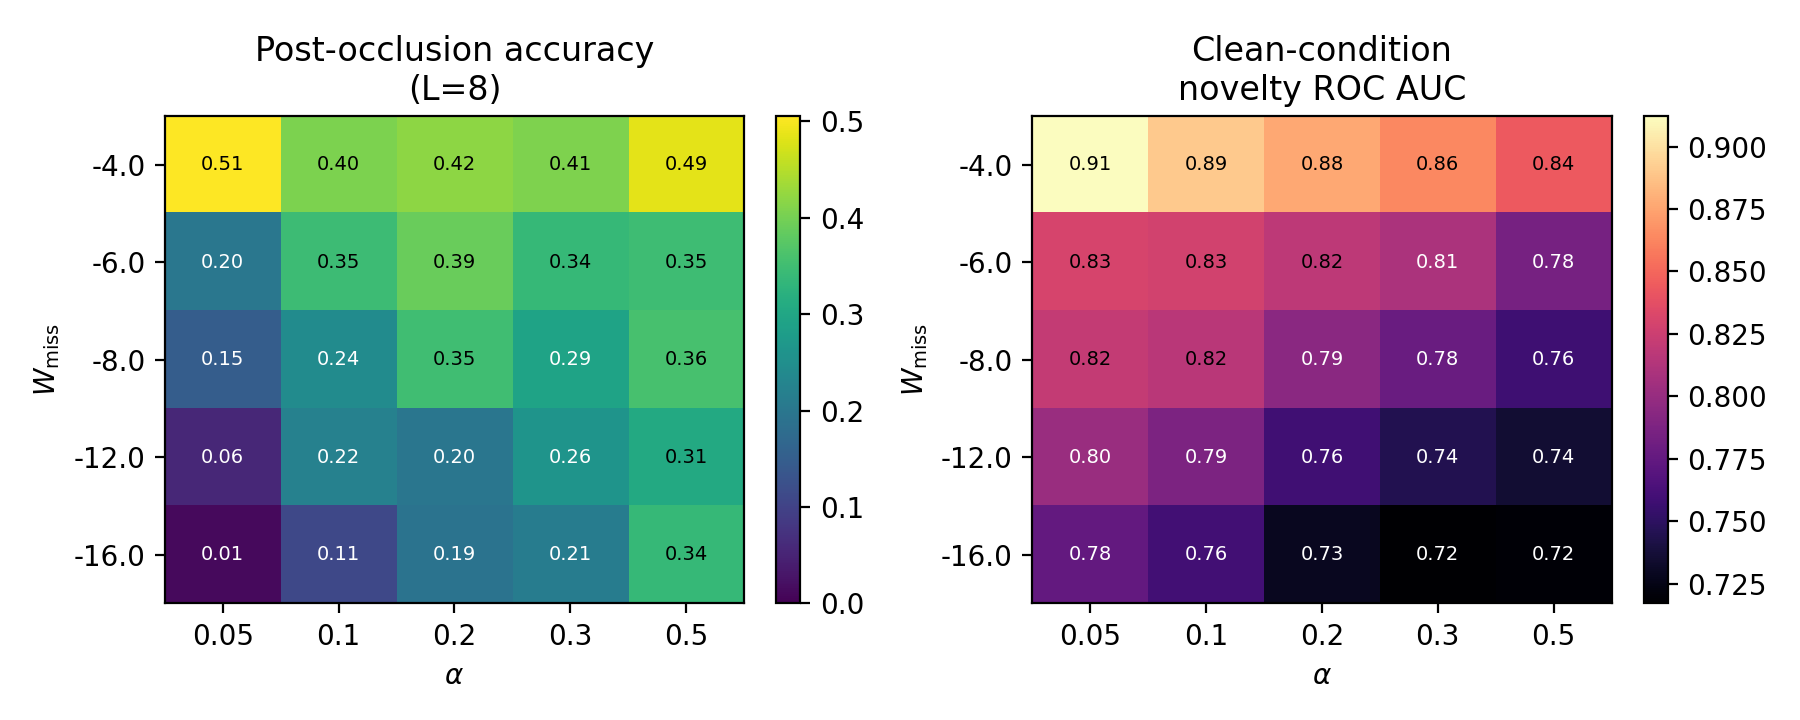
\includegraphics[width=0.85\columnwidth]{images/fig_joint_sensitivity_grid.png}
\caption{Joint $(\alpha,W_{\text{miss}})$ grid at $L=8$, $\tau_{\text{novel}}$ recalibrated per cell ($N=100$/cell). Left: post-occlusion accuracy. Right: clean-condition novelty AUC.}
\label{fig:joint_grid}
\end{figure}

The grid surfaces an interaction the 1-D sweeps cannot: at $W_{\text{miss}}=-4.0$, accuracy is \emph{non-monotonic} in $\alpha$ ($50.5\%$ at $\alpha=0.05$, dipping to $40.5$--$40.8\%$ at $\alpha\in\{0.1,0.3\}$, rising to $48.5\%$ at $\alpha=0.5$), because per-cell threshold recalibration shifts the operating point substantially (e.g.\ $\tau_{\text{novel}}$ from $-3.20$ at the paper's default to $-2.03$ at $(0.05,-4.0)$), changing how much post-occlusion error is UNKNOWN-miss vs.\ true misclassification.

\textbf{On the apparent contradiction with the recommended default.} The cell $(\alpha,W_{\text{miss}})=(0.05,-4.0)$ achieves both higher accuracy ($50.5\%$ vs.\ $24.4\%$) and higher clean-condition AUC ($0.912$ vs.\ $0.816$) than the paper's default $(0.1,-8.0)$ at this $L=8$ point under joint recalibration -- it strictly dominates the default on both measured axes here, with no transient-robustness measurement available to explain the gap away. This is the concrete evidence behind Section~\ref{sec:introduction}'s caveat: the default is retained only because it generated Sections~\ref{sec:results}.A--\ref{sec:multiclass}'s results, not because any joint criterion shows it optimal. A smaller-$|W_{\text{miss}}|$, smaller-$\alpha$ region warrants investigation across the full range of $L$ before replacing it -- left to Section~\ref{sec:future_work}.

\section{Discussion and Conclusion}
\label{sec:conclusion}

\subsection{Risks and Limitations}
\label{sec:risks}
The primary operational risk is miscalibration: $\tau_{\text{novel}}$, $\alpha$, and $W_{\text{miss}}$ are scenario-specific, and Section~\ref{sec:joint_grid} demonstrates concretely -- not hypothetically -- that a poorly-matched configuration can make ATLAS \emph{underperform} a simpler baseline. A second risk is that the reported sensitivities were characterized independently (Section~\ref{sec:results}.G) rather than jointly (Section~\ref{sec:joint_grid}), so a deployment tuned for long-occlusion recovery could unknowingly trade away short-gap or clean-condition performance. Computational risk is low: both classifiers are $O(1)$ per-track, per-scan.

Four further limitations bound scope: ATLAS's advantage over the age-normalized baseline is conditional on occlusion length ($L\ge8$ here), with the crossover uncharacterized against clutter density or $P_D$; $(\alpha,W_{\text{miss}},\tau_{\text{novel}})$ sensitivity was swept independently except for the single joint grid of Section~\ref{sec:joint_grid}; the classification layer uses synthetic Gaussian channels rather than a validated ESM/RCS model; and while Section~\ref{sec:stochastic} shows the crossover survives one stochastic (Markov) occlusion episode under an imprecisely-calibrated threshold, multi-episode or partial-fade patterns remain untested.

\subsection{Conclusion}
We introduced ATLAS, a sequence-scoring layer that eliminates infinite memory ruin by replacing an unbounded cumulative log-likelihood accumulator with an EMA and a capped survival penalty ($W_{\text{miss}}=-8.0$). Section~\ref{sec:derivation} derives a closed-form time-to-recover directly from the EMA recursion, predicting that ATLAS's recovery time remains uniformly bounded in occlusion length $L$ while the cumulative accumulator's grows without bound. This prediction is confirmed both analytically and empirically. Analytically, after accounting for the effective post-occlusion detection rate, the model matches simulation within ~2 scans for $L\le8$, with larger-$L$ gaps driven mainly by simulation right-censoring. Empirically, ATLAS recovers in a mean of $19.7$ scans at $L=8$, whereas the fixed-threshold baseline never recovers (Table~\ref{tab:ttr_combined}). At a 1~Hz scan rate, this is the difference between permanently losing custody of a track's identity and reacquiring it within roughly 20 seconds of occlusion ending. Age-normalized accumulators retain a minor advantage over brief gaps ($L\le6$); ATLAS is superior for extended signal loss ($L\ge8$), while maintaining open-set zero-day isolation via a calibrated novelty boundary. As Section~\ref{sec:joint_grid} shows, this advantage is not free of calibration risk, and the paper's default hyperparameters should be understood as the setting used to produce the reported qualitative results rather than as a jointly-optimized operating point.

\section{Future Work}
\label{sec:future_work}
\begin{enumerate}
    \item \textbf{Right-censoring-aware recovery-time model.} Section~\ref{sec:derivation} shows that from $L=8$ onward a growing fraction of trials ($43\%$ at $L=8$, $56\%$ at $L=12$, $82\%$ at $L=16$) never recover within the tested 50-scan budget, so Table~\ref{tab:ttr_combined}'s ``mean time-to-recover'' is increasingly dominated by right-censoring rather than genuine first-passage times at longer occlusions, and is not directly comparable to $n^\ast(L)$, which assumes eventual recovery. A longer simulation budget, or a survival-analysis reformulation reporting $P(\text{recovered by scan }n)$, would let $n^\ast(L)$ be validated against the quantity it actually predicts.
    \item \textbf{Adaptive fading memory and richer signatures.} Explore state-dependent $\alpha(k)$ driven by JIPDA existence probability, gating outcomes, or clutter density, retaining historical weight during brief dropouts while accelerating recovery on re-emergence; separately, isolate whether the short-gap crossover's disappearance in Section~\ref{sec:multivariate} is driven by per-scan information content or threshold recalibration, extend to non-Gaussian ESM/Swerling-type RCS signatures, and characterize how $M$ and class separation jointly affect the crossover beyond the single point tested in Section~\ref{sec:multiclass}.
    \item \textbf{Multi-objective co-calibration and real-world validation.} Section~\ref{sec:joint_grid}'s grid shows the current default is not demonstrated Pareto-optimal; a framework jointly optimizing $(\alpha,W_{\text{miss}},\tau_{\text{novel}})$ across occlusion lengths, with a direct measurement of single-scan transient robustness, is needed to responsibly select or replace it. Section~\ref{sec:stochastic}'s stochastic-occlusion result should also be recalibrated at its own scan horizon rather than reusing an earlier threshold, and extended to recorded or semi-synthetic sensor data with multi-episode or partial-fade dropout patterns rather than a single Markov episode.
\end{enumerate}

\section*{Data, Code, and Acknowledgments}
The complete Monte Carlo environment - JIPDA tracking, feature generators, and ATLAS scoring modules - is open-source at \url{https://github.com/bananajoemama/ATLAS}, parameters per Table~\ref{tab:sim_params}. The author thanks Dr. Kuo-Chu Chang for his initial review and advice on this work. The author also thanks the Sensors Directorate, Air Force Research Laboratory (AFRL) for the introduction to the foundational concepts (during the summer of 2026) in this work. All views and conclusions expressed herein are solely those of the author and do not represent the official position of the U.S. Air Force or the Department of Defense. 

\bibliographystyle{IEEEtran}
\small
\bibliography{references}

\end{document}
